\chapter{Электромагнитная индукция}

\section{Закон электромагнитной индукции}
\label{sec:11:1}

	В 1831 году М. Фарадей, проводя эксперимент с катушками, установил, что если
    изменить магнитный поток через контур, то в контуре появится индукционный
    ток. Магнитный поток же можно изменить двумя принципиально различными 
    способами:
	
	\begin{enumerate}
	\item
		при \( \vec{B} = \vconst \) изменять геометрию контура. Тогда
        \( S = S(t) \);
	\item
		при неизменной геометрии системы менять поле \( \vec{B} \), то есть
        \( \vec{B} = \vec{B}(t) \).
	\end{enumerate}
	
	Направление индукционного тока определяется правилом Ленца:
	\begin{quotation}
        Индукционный ток направлен так, что создаваемое им собственное магнитное
        поле направлено \textit{против изменения} внешнего поля \( \vec{B} \),
        порождающего этот ток.
	\end{quotation}
	
	\textit{картинка, где поле увеличивается}
	
	\textit{картинка, где поле уменьшается}
	
	Появление индукционного тока в контуре с конечным сопротивлением означает,
    что в контуре наводится ЭДС. Фарадей установил следующее отношение,
    названное \textit{законом электромагнитной индукции} в формулировке Фарадея:
	\begin{equation}
		\EDS_{\textit{инд}} = - \frac{\dd \Phi}{\dd  t}.
        \label{eq11:1}
	\end{equation}
	В формуле (\ref{eq11:1}) знак “\( - \)” связан с правилом Ленца, а
    \[
        \Phi = \iint\limits_S \vec{B}\cdot\dd \vec{S}.
    \]
	
	Если мы изменяем поток \( \Phi \) первым способом , то есть меняем
    геометрию контура, при неизменном магнитном поле, то закон ЭМИ, задаваемый
    формулой (\ref{eq11:1}), выводится формально из силы Лоренца. Покажем это.
	 
    Пусть контур \( C \) как-то движется или деформируется. Рассмотрим малый
    элемент контура \( \dd \vec{l} \), находящийся в постоянном поле
    \( \vec{B} \). Тогда на свободные заряды действует сила Лоренца.
    Следовательно, существует поле сторонних сил:
	\[
        \vec{E}_{\textit{ст}} = \frac{\vec{F}_{\textit{ст}}}{q} = 
        \vec{v}\times\vec{B}.
    \]
	 
	А, по определению, работа сторонних сил  -- это ЭДС на участке:
	\[
        \dd \EDS = \vec{E}_{\textit{ст}}\cdot\dd \vec{l} = 
        (\vec{v}\times\vec{B}) \cdot\dd \vec{l}.
    \]
    
    \begin{figure}[h]
        \center
        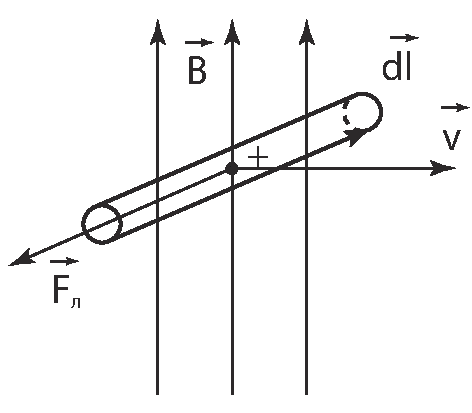
\includegraphics[width=0.3\textwidth]{lec11/emi_lorenz.pdf}
        \caption{К выводу первой части закона ЭМИ через силу Лоренца}
    \end{figure}

	Тогда во всем контуре:
	\begin{equation}
		\EDS = \oint\limits_C \vec{v}\times\vec{B}\cdot\dd \vec{l}.
        \label{eq11:2}
	\end{equation}
	
	\begin{remark}
        При \( \vec{B}(x, y, z, t) = \vconst \) и прямом проводнике длины
        \( l \), ЭДС:
        \[
            \EDS = \vec{v}\times\vec{B}\cdot\vec{l}.
        \]
	\end{remark}
	
	Покажем, что правая часть уравнения (\ref{eq11:2}) равна правой части
    уравнения (\ref{eq11:1}). Пусть \( C_1 \) и \( C_2 \) -- исходная и конечная
    геометрии контура. Его деформацию считаем малой, а изменение площади захвата
    магнитного потока контуром \( C \) равной \( \Delta S \).
	
	Тогда изменение потока при малой деформации контура из состояния \( C_1 \)
    в \( C_2 \):
	\[
        \Delta\Phi = \iint\limits_{\Delta S} \vec{B}\cdot\dd \vec{S} =
        \oint\limits_C \vec{B}\cdot\dd \vec{r}\times\dd \vec{l} =
        -\oint\limits_C \dd \vec{r}\times\vec{B}\cdot\dd \vec{l}.
    \]
	Тогда скорость изменения потока:
	\[
        \frac{\Delta\Phi}{\Delta t} =
        -\oint\limits_C \frac{\dd\vec{r}}{\dd  t}\times\vec{B}\cdot\dd\vec{l} =
        -\oint\limits_C (\vec{v}\times\vec{B})\cdot\dd \vec{l},
    \]
    что совпадает с (\ref{eq11:1}) с учетом (\ref{eq11:2}), то есть
    \[
        \EDS = -\frac{\Delta\Phi}{\Delta t}.
    \]
	
	Если мы будем изменять поток по второму способу, то формула (\ref{eq11:1})
    остается справедливой, поэтому формула (\ref{eq11:1}) является независимым
    экспериментальным законом ЭМИ.
    
    \begin{figure}[b!]
        \center
        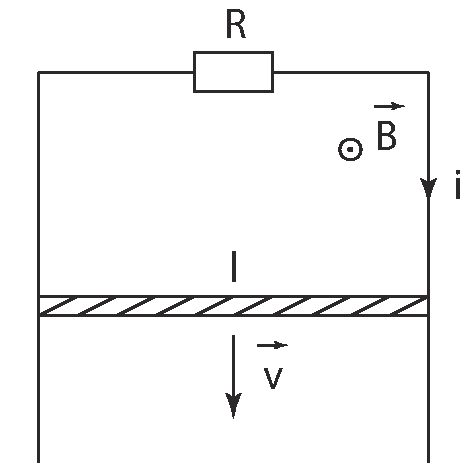
\includegraphics[width=.47\textwidth]{lec11/bridge.pdf}
        \hfill
        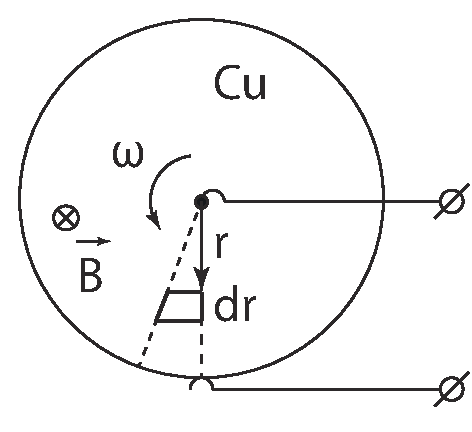
\includegraphics[width=.47\textwidth]{lec11/unipolar_generator.pdf}
        \parbox[t]{.47\textwidth}{\caption{Скользящая перемычка}}
        \hfill
        \parbox[t]{.47\textwidth}{\caption{Униполярный генератор}}
    \end{figure}	
	
    \begin{example}
        В постоянном однородном поле \( \vec{B} \) движется перемычка \( l \)
        со скоростью \( \vec{v} \). Найти ток \( i_{\textit{инд}} \) в контуре.
	\end{example}

	\begin{solution}
        \( \Phi = Blx \), где \( x \) -- текущее положение перемычки.
        Тогда ЭДС индукции может быть найдена из закона ЭМИ:
        \[
            \EDS = -\frac{\Delta\Phi}{\Delta t} = 
            -Bl\frac{\Delta x}{\Delta t} = -Blv.
        \]
        
        Тогда ток:
        \[
            i_\textit{инд} = \frac{\EDS}{R} = \frac{Blv}{R}.
        \]
	\end{solution}
	
	\begin{example}[Униполярный генератор]
	    В постоянное поле \( \vec{B} \) вращается медный диск со скоростью 
        \( \omega \). Определить \( \EDS \) на участке \( 1\rightarrow2 \).
	\end{example}
	
	\begin{solution}
        В элементе \( \dd r \) наводится ЭДС
        \[
            \dd \EDS = vB\dd  r = \omega rB\dd r.
        \]
        Следовательно, ЭДС на всём участке:
        \[
            \EDS_{1\rightarrow2} = \int\limits_0^R \omega Br\dd  r = 
            \frac{\omega BR^2}{2}.
        \]
        
        Пусть \( \omega = 10^3 \text{рад}/\text{с} \), \( R = 0,1 \text{м} \),
        \( B = 0,1 \text{Тл} \). Тогда
        \[
            \EDS = \frac{10^3 \text{рад}/\text{с} \cdot 0,1\text{Тл} \cdot
            0,1^2\text{м}^2}{2} = 0.5 \text{В}.
        \]
	\end{solution}
	
\section{Вихревое электрическое поле}

    Если геометрия контура не меняется, а поле \( \vec{B} \) зависит от времени
    \( \vec{B} = \vec{B}(x, y, z, t) \), то в контуре появляется ЭДС:
    \[
        \EDS = \oint\limits_C \vec{E}_{\textit{ст}}\cdot\dd \vec{l} = 
        -\frac{\dd \Phi}{\dd  t} = 
        -\frac{\dd }{\dd  t} \iint\limits_S \vec{B}\cdot\dd \vec{S} = 
        -\iint\limits_S \frac{\partial\vec{B}}{\partial t}\cdot\dd \vec{S}.
    \]
    Сторонняя сила в этом случае:
	\[
        \vec{E}_{\textit{ст}} = \frac{\vec{F}_{\textit{ст}}}{q}.
    \]
	
    Максвелл предположил, что поле сторонних сил \( \vec{E}_{\textit{ст}} \) --
    это “обычное” электрическое поле в том смысле, что его действие на заряды 
    такое же, как и у обычного электрического поля \( \vec{E} \). Это поле 
    \( \vec{E}_{\textit{ст}} \) названо \textbf{вихревым} электрическим полем.
    Его линии, в отличие от линий поля \( \vec{E} \) не имеют источников.
	
	Тогда закон ЭМИ в формулировке Максвелла:
	\begin{equation}
		\oint\limits_C \vec{E}_{\textit{в}}\cdot\dd \vec{l} =
        - \iint\limits_S \frac{\partial\vec{B}}{\partial t}\cdot\dd \vec{S}.
        \label{eq11:3}
	\end{equation}
	
    Звучит он так: изменение потока магнитного поля \( \vec{B} \) через контур
    порождает вихревое электрическое поле, связанное с полем \( \vec{B} \)
    формулой (\ref{eq11:3}), где ориентированная поверхность \( \dd \vec{S} \)
    и обход контура образуют правый винт.
	
	Формулу (\ref{eq11:3}) можно записать в дифференциальном виде,
    воспользовавшись теоремой Стокса:
	\[
        \oint\limits_C \vec{E}_{\textit{в}}\cdot\dd \vec{l} = 
        \iint\limits_S \rot\vec{E}_{\textit{в}}\cdot\dd \vec{S}.
    \]
	А так как поверхность \( S \) произвольна, то из (\ref{eq11:3}) получаем:
	\begin{equation}
		\rot\vec{E}_{\textit{в}} = -\frac{\partial\vec{B}}{\partial t}
        \label{eq11:3a}
	\end{equation}
	
	Формула (\ref{eq11:3a}) означает, что если поле \( \vec{B} \) меняется в
    данной точке пространства, то в данной точке пространства есть вихревое
    поле \( \vec{E}_{\textit{в}} \).
	
\section{Проявления электромагнитной индукции}
    \begin{figure}[b!]
        \center
        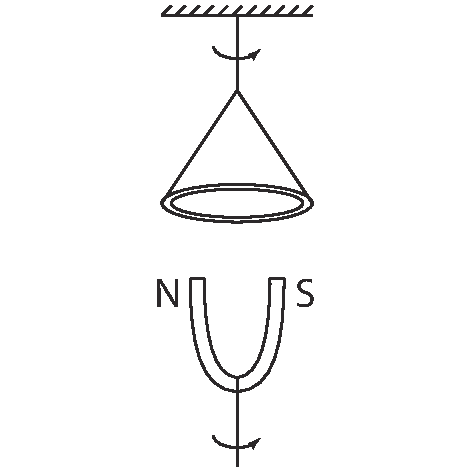
\includegraphics[width=.47\textwidth]{lec11/engine_model.pdf}
        \hfill
        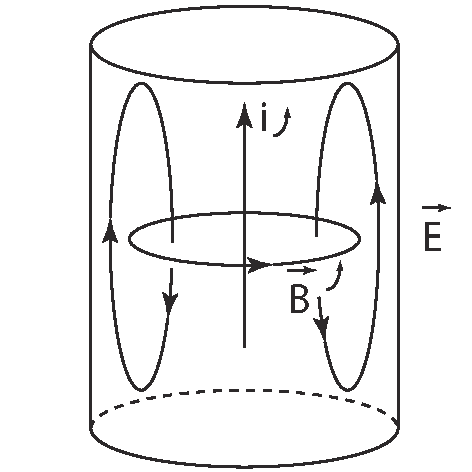
\includegraphics[width=.47\textwidth]{lec11/skin_effect.pdf}
        \parbox[t]{.47\textwidth}{\caption{Модель асинхронного двигателя --
            контур во вращающемся магнитном поле}}
        \hfill
        \parbox[t]{.47\textwidth}{\caption{Скин-эффект}}
    \end{figure}

	\begin{enumerate}
	\item Вихревые токи (токи Фуко).
	
	\item Висящее кольцо.
	
	\item Модель асинхронного движгателя.
	
	\item  Скин-эффект -- явление вытеснения тока к поверхности проводника при высоких частотах.
	\end{enumerate}

